\section{State of the Art}

\subsection{Semantic Segmentation}

The segmentation of wounds belongs to the class of semantic segmantation problems, where a pixel-wise classification is performed. In the case of wound segmentation there are two classes: foreground, which is the wound, and background. Deep Learning methods became dominant in the last years because they became more accessible. Fully Convolutional Neural Networks (fCNN) as a starting point in research had the drawback of resulting in a low output resolution and multiple techniques were invented to increase the output resolution \cite{Litjens2017}. This results in an encoder-decoder architecture as base for the networks, inspired by auto-encoders \cite{linknet}, where the encoder subsamples and the decoder upsamples \cite{Norelyaqine2023}. In such architectures the encoder generates context information, information in the feature space while the decoder maps this information into the spatial context.

Pre-training for such models requires a huge amount of data. A typical data set for such pre-training is the ImageNet object classification data set \cite{SegNet}.

In this project, four different segmentation models are used: U-Net, Linknet, FPN and PSPNet. All are improved architectures about a basic fCNN. Each architecture is described in detail to understand challenges and approaches of localizing information in space.

\paragraph{U-Net}

U-Net is a convolutional network developed for Biomedical Image Segmentation, based on an encoder-decoder architecture. Encoder and decoder are called contracting and expansive path in the original paper, describing their function. They are also described as context path and spatial path \cite{MO2022626}. Both, encoder and decoder consist of different steps to encode and decode the image on different spatial levels. The encoder is a classical CNN; each step consists of two convolutions and a max pooling operation for downsampling. The decoder step upsamples the feature map followed by a convolution. The result is then concatenated with the corresponding feature map from the encdoer path and convolution is applied again. In the final layer, 1x1 convolution is used to map the feature vector to the desired number of classes. This architecture is visualised in figure \ref{fig:unet-architecture}. \cite{unet}

\begin{figure}[htb!]
	\centering
	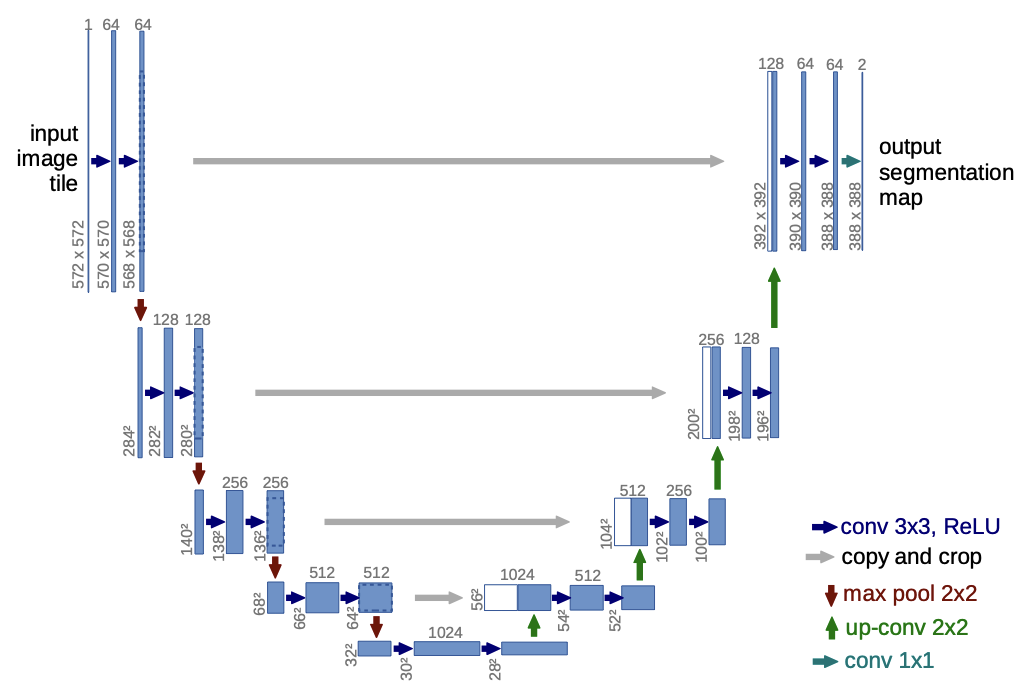
\includegraphics[width=0.8\textwidth]{fig/unet-architecture.png}
	\caption{U-Net architecture for 32x32 pixels in the lowes resolution. Blue boxes are feature maps with the number of feature-channels on top of the boxes and the size shown on the left size. Operations are indicated by the arrows. The skip connections are a concatenation. The figure originally create by \citeauthor{unet} \cite{unet}.}
	\label{fig:unet-architecture}
\end{figure}

The skip connections, connecting the different levels of encoder and decoder prevent a loss of information and extracting the features at different resolutions to retrieve spatial information. By doing this, it is one of the first architectures improving the classical fCNN for semantic segmantation \cite{Litjens2017}. While U-Net provides spatial localization of features, its ability to generalize to multi-scale information is limited \cite{Norelyaqine2023}.

One restriction is, that the input size must be chosen such that all 2x2 max-pooling operations in the encoder are applied to an even x and y size.


\paragraph{Linknet}

Similar to U-Net, Linknet contains of an encoder block for downsampling and a decoder block for upsampling. The downsampling is not done by max pooling as it is in the U-Net architecture but by using a stride of 2 in a convolutional layer. Also does the inital encoder block differ from the following blocks as it uses a larger kernel and uses max pooling. The decoder blocks upsample by a factor of 2 in each block. The final block differs again from the previous blocks. The main difference to the U-Net architecture is how the skip connections are used: Similarly to the U-Net, there are skip connections between the corresponding steps of encoder and decoder, but the feature map from the encoder is not concatenated but added to decoder data. The linknet architecture is visualised in figure \ref{fig:linknet-architecture}. \cite{linknet}

\begin{figure}
	\centering
	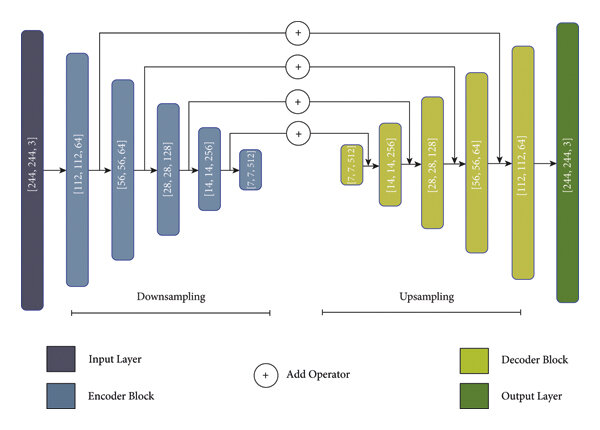
\includegraphics[width=0.8\textwidth]{fig/linknet-architecture.jpg}
	\caption{A visualisation of the LinkNet architecture originally provided by \citeauthor{Norelyaqine2023} \cite{Norelyaqine2023}.}
	\label{fig:linknet-architecture}
\end{figure}


%\begin{itemize}
%	\item "LinkNet sends spatial information directly from the encoder to the matching decoder, conserving as much of the image’s spatial information as feasible."
%	\item "directly connects shallow feature map in encoder module to the decoder module of the corresponding size" $\rightarrow$ accurate position information on shallow layer, avoids redundant parameters and computations \cite{Norelyaqine2023}
%\end{itemize}

The implementation used in this project has four skip connections instead of the original three \cite{SegmentationModels}. Similarly to the U-Net, the input size is restricted such that every upsampling operations need to be applied to an even x and y size.

\paragraph{FPN}

\begin{itemize}
	\item long for Feature Pyramid Network
	\item creating feature maps of various layers and sizes \cite{Norelyaqine2023}
	\item bottom-up pathway: "feature hierarchy consisting of feature maps at several scales with scaling step of 2"\cite{fpn}
	\item top-down-pthway and lateral connections": "higher resolution features by upsampling spatially coarser, but semantically stronger, fea- ture maps from higher pyramid levels", enhance with features from bottom-up pathway via lateral connections $\rightarrow$ merge feature maps of same spatial size from both pathways\cite{fpn}
	\item bottom-up feature map: lower-level sementatics but activations more accurately localized (fewer subsampling)\cite{fpn}
	\item creation of top-down feature maps: upsample and then merge\cite{fpn}
	\item final feature contains local and global context information\cite{fpn}
\end{itemize}


\paragraph{PSPNet}

\begin{itemize}
	\item long for Pyramid Scene Parsing Network
	\item feature map extracted with pretrained backbone
	\item pyramid pooling to get context information
	\item pyramid pooling: fusion of features under four different pyramid scales (global pooling and sub-regions for different locations), 1x1 convolution to maintain weight of global feature after each pyramid, upsampling of output to get same size as original feature map
	\item "different levels of features concatenated as final pyramid pooling feature"
	\item final prediction by convolution layer which input isoriginal feature map concatenated with pyramid pooling output
	\item motivation: pyramid pooling provides levels of information, more helpful than global pooling
\end{itemize}

\subsubsection{Evaluation}

There exist several methods to evaluate how good a predicted segmentation is. Since semantic segmentation performs a pixel-wise classification, resulting in a segmentation mask, classical metrics such as accuracy and precision are available. Two performance metrics that are commonly used in semantic segmentation in medical imaging are the Dice Coefficient and the Intersetcion over Union (IoU) score. They indicate the segmentation quality better than pixel-wise accuracy \cite{Eelbode}.

\paragraph{IOUScore}

The IoU-Score (Intersection over Union), also known as the Jaccard index $J$ describes the ratio between the intersection of the ground truth mask $y$ and the predicted mask $\tilde{y}$ and the union of the predicted and the ground truth mask. By this it compares the similarity of the two masks \cite{Cho2021WeightedIO}.

\begin{align}
	\text{IoU}(y, \tilde{y} :&= \frac{\text{Area of overlap}}{\text{Area of union}}\\
	&=\frac{|y \cap \tilde{y}|}{|y \cup \tilde {y}|}
\end{align}


\paragraph{Dice Coefficient}

The Dice coefficient is the F1 score calclulated for the image masks. In terms of intersection and union, this means it calculates the ratio between two times the overlap between ground truth $y$ and predicted mask $\tilde{y}$ and the total area.

\begin{align}
	\text{Dice}(y, \tilde{y}) :&= 2 \cdot \frac{\text{Area of overlap}}{\text{Total area}}\\
	&= 2 \cdot \frac{|y \cap \tilde{y}|}{|y| + |\tilde{y}|}
\end{align}

To gain more insight into the type of the errors the model makes, the rate of false positives and false negatives can be used do differentiate Type I and Type II errors \cite{DFUC2022}.

% "The difference between the two metrics is that the IoU penalizes under- and over-segmentation more than DSC"

\subsubsection{Loss function}

\begin{itemize}
	\item loss function often uses pixel-wise (weighted) cross-entropy loss even though differentiable approximations of the two metrics exist \cite{Eelbode}
\end{itemize}

% DiceLoss is used in the code

\subsubsection{Data Augmentation}

\begin{itemize}
	\item augmentation useful especially if available data is limited
	\item makes it more robust and accurate
	\item augmentations can be divided in two categories: position augmentation and color augmentation
	\item what augmentations are appropriate for the application
\end{itemize}

% https://nanonets.com/blog/data-augmentation-how-to-use-deep-learning-when-you-have-limited-data-part-2/
% https://www.v7labs.com/blog/data-augmentation-guide


\subsection{Wound Segmentation}

% What are wounds that need to be segmented? Focus on chronic wounds
\begin{itemize}
	\item one type: diabetic foot ulcers $\rightarrow$ are monitored to ensure healing process is optimal and there is no infection, normally long time span \cite{DFUC2022}
\end{itemize}

% Why is wound segmentation a more complex segmentation problem
\begin{itemize}
	\item wounds have complex structure containing different types of tissue with different colour and texture $\rightarrow$ different regions with borders in between \cite{AhmadFauzi2015}
	\item heterogeneous wound images
\end{itemize}

% what models do exist by now, what is the sota
\begin{itemize}
	\item before deep networks: features describing color and texture, algorithms such as region growing and optimal thresholding or classical machine learning models, e.g. Support Vector Machines \cite{Scebba2022}
	\item Convolutional Neural Networks then used, manually extracted features replaced by the ones the CNN learns autonomously \cite{Scebba2022}
	\item some methods include pre-processing steps to remove background (User interaction, manual feature engineering to detect background pixels, standardizing background in advance before taking feature) $\rightarrow$ not automatic
	\item Diabetic Foot Ulcer Challenge 2022 used FCN, U-Net and SegNet with different backbones as baseline for their challenge (categorical cross-entropy loss) \cite{DFUC2022}
	\item generally often classical models used with minor adaptions
	\item following standing out
	\item \citeauthor{Scebba2022} proposed two step method: object detector that produces bounding boxes containing the wounds and then segmentation on those areas (u-net, convNet, DeepLapV3 with ResNet-101 backbone and FCN with VGG16 backbone, pixel-wise weighted binary cross entropy loss, weighting term was computed as the ratio between the total number of wound bed and background pixels of each training set fold)
	\item \citeauthor{Oota_2023_WACV} claim they set a new state of the art, their method will described in more detail in the following
\end{itemize}


\subsubsection{WSNET}

\begin{itemize}
	\item based on the four before described segmentation architectures: U-Net, LinkNet, PSPNet and FPN
	\item experimented with different backbones, in the scope of this project MobileNet \cite{howard2017mobilenets} is used since it is the smallest one and allows faster training
	\item all backbones with ImageNet pre-trained weights
	\item they performed Wound-Domain Adaptive Pretraining by classifying the wound images in 5 ulcer types
	\item data augmentation on the training data and corresponding masks, not on test data
	\item augmentation consists of horizontal flip, random rotation, optical distortion, grid distortion, blur, random brightness contrast, and transpose
\end{itemize}

\paragraph{Global-Local Architecture}

\begin{itemize}
	\item motivation: obtain global signals from entire image and local signals from smaller patches for details
	\item only local might cause incomplete segmentation for large wounds
	\item local architecture: split image in 16 non-overlapping patches (48x48x3), stacking results in 48x48x(3x16) volume
	\item parallel 16 local models with shared weights
	\item combined to full-size mask at end
	\item stack output of global and local model to output of size (192x192x2)
	\item 1x1 convolution to get final mask
\end{itemize}

% own judgement of method
\begin{itemize}
	\item interesting that they use segmentation models that already use methods to localize method, e.g. FPN already considers different context sizes
	\item chosen patch size implies some property of the wound images, which size is important for local information
	\item they stated in their paper that they tested different patch sizes and chose 48 because it lead to the best results
\end{itemize}


\paragraph{Reported Results}

\begin{itemize}
	\item pretraining on wound images improves results
	\item data augmentation leads to improvements
	\item local only models significantly worse than global model
	\item global only models worse than global-local model
\end{itemize}



